%% Version 4.3.2, 25 August 2014
%
%%%%%%%%%%%%%%%%%%%%%%%%%%%%%%%%%%%%%%%%%%%%%%%%%%%%%%%%%%%%%%%%%%%%%%
% Template.tex --  LaTeX-based template for submissions to the 
% American Meteorological Society
%
% Template developed by Amy Hendrickson, 2013, TeXnology Inc., 
% amyh@texnology.com, http://www.texnology.com
% following earlier work by Brian Papa, American Meteorological Society
%
% Email questions to latex@ametsoc.org.
%
%%%%%%%%%%%%%%%%%%%%%%%%%%%%%%%%%%%%%%%%%%%%%%%%%%%%%%%%%%%%%%%%%%%%%
% PREAMBLE
%%%%%%%%%%%%%%%%%%%%%%%%%%%%%%%%%%%%%%%%%%%%%%%%%%%%%%%%%%%%%%%%%%%%%

%% Start with one of the following:
% DOUBLE-SPACED VERSION FOR SUBMISSION TO THE AMS
%\documentclass{ametsoc}


% TWO-COLUMN JOURNAL PAGE LAYOUT---FOR AUTHOR USE ONLY
\documentclass[twocol]{ametsoc}


%%%%%%%%%%%%%%%%%%%%%%%%%%%%%%%%
%%% To be entered only if twocol option is used

\journal{jcli}

%  Please choose a journal abbreviation to use above from the following list:
% 
%   jamc     (Journal of Applied Meteorology and Climatology)
%   jtech     (Journal of Atmospheric and Oceanic Technology)
%   jhm      (Journal of Hydrometeorology)
%   jpo     (Journal of Physical Oceanography)
%   jas      (Journal of Atmospheric Sciences)	
%   jcli      (Journal of Climate)
%   mwr      (Monthly Weather Review)
%   wcas      (Weather, Climate, and Society)
%   waf       (Weather and Forecasting)
%   bams (Bulletin of the American Meteorological Society)
%   ei    (Earth Interactions)

%%%%%%%%%%%%%%%%%%%%%%%%%%%%%%%%
%Citations should be of the form ``author year''  not ``author, year''
\bibpunct{(}{)}{;}{a}{}{,}

%%%%%%%%%%%%%%%%%%%%%%%%%%%%%%%%

%%% To be entered by author:

%% May use \\ to break lines in title:

\title{Global Optimization of the Analogue Method by Means of Genetic Algorithms}

%%% Enter authors' names, as you see in this example:
%%% Use \correspondingauthor{} and \thanks{Current Affiliation:...}
%%% immediately following the appropriate author.
%%%
%%% Note that the \correspondingauthor{} command is NECESSARY.
%%% The \thanks{} commands are OPTIONAL.

    %\authors{Author One\correspondingauthor{Author One, 
    % American Meteorological Society, 
    % 45 Beacon St., Boston, MA 02108.}
% and Author Two\thanks{Current affiliation: American Meteorological Society, 
    % 45 Beacon St., Boston, MA 02108.}}

\authors{Pascal Horton\correspondingauthor{Terranum, Rue de l'industrie 35 bis, 1030 Bussigny, Switzerland.}}

%% Follow this form:
    % \affiliation{American Meteorological Society, 
    % Boston, Massachusetts.}

\affiliation{University of Lausanne and Terranum, Lausanne, Switzerland}

%% Follow this form:
    %\email{latex@ametsoc.org}

\email{pascal.horton@alumnil.unil.ch}

%% If appropriate, add additional authors, different affiliations:
    %\extraauthor{Extra Author}
    %\extraaffil{Affiliation, City, State/Province, Country}

\extraauthor{Michel Jaboyedoff}
\extraaffil{University of Lausanne, Lausanne, Switzerland}

%% May repeat for a additional authors/affiliations:

%\extraauthor{}
%\extraaffil{}

\extraauthor{Charles Obled}
\extraaffil{Universit\'{e} de Grenoble-Alpes, LTHE, Grenoble, France}

%%%%%%%%%%%%%%%%%%%%%%%%%%%%%%%%%%%%%%%%%%%%%%%%%%%%%%%%%%%%%%%%%%%%%
% ABSTRACT
%
% Enter your abstract here
% Abstracts should not exceed 250 words in length!
%
% For BAMS authors only: If your article requires a Capsule Summary, please place the capsule text at the end of your abstract
% and identify it as the capsule. Example: This is the end of the abstract. (Capsule Summary) This is the capsule summary. 

\abstract{The analogues method is based on a statistical relationship between synoptic atmospheric variables and local weather, which we aim at forecasting. This relationship is expressed through many parameters that are usually calibrated by means of a semi-automatic procedure. This sequential calibration is relatively fast and provide acceptable results, but it has strong constraints, is made of successive steps and thus cannot handle parameters dependencies, and mainly, it cannot calibrate automatically some parameters, such as the selection of the pressure levels and the temporal windows on which the predictors are compared. In order to surpass these limitations, we assessed a global optimization technique, namely genetic algorithms, that can optimize jointly all parameters of the method and thus provide a global optimum by taking into account the parameters dependencies. Moreover, it can calibrate parameters that were previously manually assessed, and can take into account new degrees of freedom that were unthinkable before. 
	The global optimization can optimize all parameters jointly and automatically, which is a breakthrough in the way the analogue method was calibrated until now. Indeed, it allows taking into account parameters inter-dependencies, adding new degrees of freedom, and choosing objectively some parameters that were manually selected beforehand (such as the pressure levels and the temporal windows of the predictor variables).
	These kind of optimization techniques need however to be tailored to the problem to solve. We had to assess multiple combinations of algorithms, and even to develop new operators, such as the \textit{chromosome of adaptive search radius} which was found to be very robust, in order to make recommendations for the use of genetic algorithms to optimize the analogue method. These recommendations are a consequent outcome of this work, as it opens new perspective for the improvement of the analogue method, and its application to new regions or to new predictands.
	}

\begin{document}

%% Necessary!
\maketitle


%%%%%%%%%%%%%%%%%%%%%%%%%%%%%%%%%%%%%%%%%%%%%%%%%%%%%%%%%%%%%%%%%%%%%
% MAIN BODY OF PAPER
%%%%%%%%%%%%%%%%%%%%%%%%%%%%%%%%%%%%%%%%%%%%%%%%%%%%%%%%%%%%%%%%%%%%%
%

%% In all cases, if there is only one entry of this type within
%% the higher level heading, use the star form: 
%%
% \section{Section title}
% \subsection*{subsection}
% text...
% \section{Section title}

%vs

% \section{Section title}
% \subsection{subsection one}
% text...
% \subsection{subsection two}
% \section{Section title}

%%%
% \section{First primary heading}

% \subsection{First secondary heading}

% \subsubsection{First tertiary heading}

% \paragraph{First quaternary heading}


\section{Introduction}
\label{section_intro}





The sequential calibration cannot optimize all parameters of the AM, as several are manually selected, such as the meteorological variable, the pressure level and the temporal windows. Testing multiple combinations of these can be cumbersome, especially when considering multiple predictors within the same level of analogy. Moreover, the parameters are calibrated successively within the same level of analogy, and in-between them.

 This article is not about discussing the results of such a technique, but describing the details of the implementation. The demonstration of the benefit brought by such an approach is the topic of another article. 





Up to now, the optimization of the method has been undertaken by semi-automatic calibration procedures. However, the choice of predictor variables, pressure levels and temporal windows were still to be chosen manually before optimizing the spatial windows and the number of analogues. Moreover, the semi-automatic technique proceeds to the optimization sequentially, ignoring potential dependencies between the parameters of the method. Thus, optimizing the method with the semi-automatic technique is laborious, as many combinations of predictors (variables, pressure levels, temporal windows) have to be assessed. Moreover, due to its sequential approach, the risk of ending in a local optimum is high and can not be avoided. We thus propose a global optimization approach by means of Genetic algorithms, tailored to the analogue method (AM).



\section{The analogue method}
\label{section_analog_method}



\section{Motivation for a global optimization}

The classic calibration is fast to optimize one spatial window for a given pressure level and temporal window. However, it doesn't provide an objective selection of the pressure level and temporal window. The only option is to try systematically every combination, which may be acceptable for no more than 2 levels. However, \citet{Horton2012a} showed that additional pressure levels may improve the method.

We observed during the calibration of the analogue method that the resulting parameters vary with the initial choices (such as the number of analogues). In addition, the different levels of analogy (eg on the atmospheric circulation and the moisture index) are always calibrated sequentially. However, we can not exclude any dependency between them, which could lead us to select another parametrization if we calibrate them together. Simultaneous calibration of all parameters has never been undertaken so far. Only a global optimization technique can be able to optimize all parameters of all analogy levels simultaneously.

When creating the classic calibration procedure, \citet{Bontron2004} was aware of the problem of dependencies between parameters and wrote: '' \textit{We perceive here the combinatorial aspect of our problem: variables and spatial windows are not independent. We will present our results by first searching the best variable [note: e.g. selection of the pressure level and the temporal window for the geopotential height] on a chosen spatial window, and next, the best window for the chosen variable. However, even by repeating the process, are we sure to obtain the optimal combination?} ''. And later in his work: '' \textit{Our approach, which is again to vary the parameters one by one -- the others being fixed in a more or less arbitrary manner -- may therefore not exactly lead us to the optimal solution} ''. \citet{Bliefernicht2010} has also faced the combinatorial issue of the parameters of the analogue method and concludes that one needs to be an expert to know their respective influence, their sensitivity and their nonlinear interactions. \citet{BenDaoud2010}, when calibrating the analogue method, also stated that '' \textit{the combinatory aspect related to the calibration was found to be too high for all the parameters to be calibrated simultaneously } ''.

The analogue method needs to be adapted to every new region it is applied, because the leading meteorological influences are specific to this region. Even the selection of the pressure level and the temporal window should be reconsidered, when not the variable itself. For example, \citet{BenDaoud2010} found the vertical velocity relevant for the great plains in France, when \citet{Horton2012a} found no interest in this variable in an Alpine environment, because in the Alps, the vertical motion is mainly controlled by orographic effects, and was thus already well related to the atmospheric circulation itself. So, when adapting the analogue method to a new region, we should assess systematically every combination of pressure levels, time and spatial windows, which is an intensive task. This procedure can be automatized by a global optimization technique.

Our ambition was then to assess the feasibility of an automatic optimization of the analogue method through various techniques. The objective was to find an approach to optimize all parameters simultaneously, and thus be able to identify the global optimum in the parameter space. In addition, it can overcome the systematic manual assessments of certain parameters such as the selection of the pressure levels and time windows. Finally, it can open new perspectives by allowing the addition of new degrees of freedom, such as a weighting of the criteria values between the pressure levels, and the consideration of non-overlapping spatial windows between the pressure levels.

\citet{Horton2012a} assessed the ability of the \citet{Nelder1965a} method based on a simplex approach. This technique didn't provide satisfying results and failed at identifying the global optimum. Indeed, the results didn't converge and many local optimums came out. The parameter space of the analogue method is very complex and not appropriate for a linear optimization technique. Genetic algorithms were found to be much more relevant for such application.


\section{Assessed Genetic Algorithms variants}
\label{sec:gas}

Genetic Algorithms (GAs) come from the world of stochastic optimization, more specifically from metaheuristic approaches. These are stochastic iterative algorithms that behave like search algorithms by exploiting the characteristics of a problem and are particularly suitable for complex parameter spaces.

Genetic algorithms are part of the family of evolutionary algorithms \citep{Back1993b, Schwefel1993}, which get inspiration from some mechanisms of biological evolution, such as reproduction, genetic mutations, chromosomal crossovers, and natural selection. GAs are the most used technique from evolutionary algorithms \citep{Back1993b}, and they are constantly improving \citep{Haupt2004}. However, with time, the different methods of evolutionary algorithms tend to be similar and share many commonalities \citep{Back1996b, Haupt2004}.

The method was originally developed by \citet{Holland1992b} and popularized by \citet{Goldberg1989}. Unlike a linear or local optimization, GAs seek the global optimum on a complex surface, theoretically without restriction, but with no guarantee to reach it.


\subsection{Basic concepts of the genetic algorithms}

GAs mimic the evolution of a population of individuals in a new environment, by applying rules based on natural processes, such as DNA mutation, chromosomes crossover, natural selection, etc. It simulates the fact that in a natural environment, the most suitable individuals tend to survive longer, to reproduce more easily, and so to influence coming generations by providing genes that provide some good performance in a certain domain. Generation after generation, the DNA mixes and the strong genes cumulate in some individuals \citep{Beasley1996a}. Globally, the fitness of the population to its environment increases, while retaining enough variety to not converge too quickly to a local optimum.

Applications of GAs are very diversified as they can handle many parameters of various types \citep{Joines1996a}, even with very complex cost surfaces \citep{Haupt2004}. GAs work remarkably well with intervariable dependences \citep{Haupt2004}. The objective function to optimize (often named fitness function in this context) can be of different types (mathematical function, experimental or numerical modeling). Only the resulting value is used for optimization. Indeed, these algorithms do not require any knowledge of the problem, which can be used as black-box, but they must be adapted in order to perform optimally.

By means of the reproduction operator and the natural selection, the GAs focus on the most promising regions of the parameter space \citep{Holland1992b}. Points (parameter sets) are densified in these areas because the strong genes of the best individuals propagate from generation to generation.

Two conditions guarantee in theory the convergence to the global optimum \citep{Zitzler2004a}: (1) Parameters mutations that can allow to explore the entire parameter space, thereby ensures that any value can be achieved with a non-zero probability. (2) A rule of elitism ensuring that an optimal solution cannot be lost or damaged.


\subsection{Structure and operators}

The GAs optimize a population of individuals (parameter sets). Each individual contains a chromosome (parameters of the AM in our case). We call gene every parameter that constitutes the chromosome. The parameters to optimize have long been coded in binary form and assembled as strings in the canonical GAs \citep{Goldberg1989}. Encoding and decoding steps were needed to transform the variable from its floating-point representation into its binary representation, and vice versa, which introduce quantification errors \citep{Haupt2004}. According to \citet{Holland1992b}, working with binary chromosomes was supposed to be more efficient \citep{Goldberg1990a, Back1993b}. However, more and more applications use floating-point representations, allowing to avoid the coding and decoding steps and the quantification errors \citep{Haupt2004}, and which also often resulted in a performance improvement \citep{Goldberg1990a}. It is thus now considered that for continuous variables, a floating-point representation is more suited \citep{Michalewicz1996, Herrera1998a, Haupt2004, Back1996b, Gaffney2010a}. 

There are numerous implementation variants of GAs often optimal for a given problem \citep{Hart1991a,Schraudolph1992a}. The divergences are the operators implementation, through significantly different algorithms, which has an important effect on the results \citep{Gaffney2010a}. However, the structure of the method (Figure \ref{fig:structure_gas}) resulting from the work of \citet{Holland1992b} is common to most applications \citep{Back1993b}, and consists in the following steps:

\begin{enumerate}
	\item A population of $N$ individuals (parameter sets of the AM) is randomly generated, which constitutes the initial population.
	\item The fitness (performance score or objective function) of every individual is assessed.
	\item A natural selection is applied, after which only the best individuals remain, which constitutes the intermediate generation.
	\item From this intermediate generation, couples are formed according to given rules.
	\item These couples proceed to reproduction, or chromosome crossover, in order to mix their genes (parameters) according to the operator version. New children are generated in order to fill the intermediate generation back to $N$ individuals.
	\item Parents and children are then subject to mutation, where some genes get affected, meaning some parameter values are randomly changed.
	\item The new formed generation is then re-assessed.
	\item According to the ending criteria, the optimization ends or starts again for another iteration.
\end{enumerate}

\begin{figure}[htb]
	\noindent\includegraphics[width=19pc,angle=0]{figures/figure_structure_gas.pdf}\\
	\caption{Genetic algorithms operational flowchart}
	\label{fig:structure_gas}
\end{figure}

All operators we used and their options, applied to real coding, are described in the following sections. Many other operators exist, but we will only present the ones we evaluated.

\subsubsection{Genesis of the population}

The first step of the optimization is to generate the initial population. A population is a set of $N$ individuals (each of which represents a point in the space of potential solutions, a parameter set of the AM in our application) that we are going to make evolve. A generation is the population at a given time. 

A random initialization based on a uniform distribution is the most current version. The size $N$ of the population is often a compromise between the computation time and the quality of the solution. $N$ must allow sufficient sampling of the solutions field \citep{Beasley1996a}, and should thus vary as a function of chromosome size (ie the number of parameters to be optimized). 


\subsubsection{Natural selection}

Natural selection is performed on the basis of the values of the objective function. The selection allows to only keep a certain part of the population, usually half ($N/2$), which can access the mating pool (intermediate generation with $N_{mp}$ members). If $N_{mp}$ is too high, the reproduction rate is too low, whereas if it is too small, the strong traits of individuals do not have the ability to accumulate in the same chromosome \citep{Haupt2004}. Several techniques exist, such as:

\begin{itemize}
	\item \textbf{$N_{mp}$-elitism} \citep{Michalewicz1996}: the population is sorted according to the value of the objective function and only the better half is preserved. 
	
	\item \textbf{Tournament selection} \citep{Michalewicz1996, Zitzler2004a}: two individuals are randomly selected and fight. The one with the highest performance score is chosen, but with a certain probability, in order to reduce the selection pressure. This procedure is repeated until the mating pool is full. Individuals can be selected several times, and thus be represented several times in the mating pool.
\end{itemize}


\subsubsection{Selection of the couples}

Individuals of the mating pool can reproduce. It begins with the selection of pairs (the parents). The techniques implemented in this work are the following:


\begin{itemize}
	\item \textbf{Rank pairing}: individuals are gathered in pairs according to their rank (classified on the performance scores). Consecutive ranks are put together (odd rows are associated with even rows). This approach is easy to achieve, but does not look like a natural process.
	
	\item \textbf{Random pairing}: two individuals are randomly selected to form a couple, according to a uniform law.
	
	\item \textbf{Roulette wheel weighting}: the roulette technique refers to gambling. But unlike casino roulette, this one is biased. Each individual is associated with a sector of the wheel with a certain opening angle, which is its probability of selection \citep{Haupt2004}. The probability assigned to the individuals is proportional to their fitness (objective function), so that the most adapted individuals have the greatest probability of reproduction. There are two techniques for weighting the individuals of the mating pool:
	
	\textit{Roulette wheel weighting on rank}: the probability of each individual depends on its rank $n$:
	\begin{equation}
	p_{n}=\dfrac{N_{mp}-n+1}{\sum^{N_{mp}}_{n=1}n}
	\label{equation_mating_rank_weighting}
	\end{equation}
	
	\textit{Roulette wheel weighting on fitness}: the selection probability is calculated based on the value of the objective function. This approach gives more weight to the best individuals when the distribution of performance scores is wide, while the weight is almost similar when all individuals have approximately the same performance score \citep{Haupt2004}. The probability $p_{n}$ of each individual is calculated by the equation \ref{equation_mating_score_weighting}:
	\begin{equation}
	p_{n}=\frac{score_{n}-score_{N_{mp}}}{\sum_{n=1}^{N_{mp}} (score_{n}-score_{N_{mp}})}
	\label{equation_mating_score_weighting}
	\end{equation}
	In our application, the last individual ($N_{mp}$) has zero probability of being selected.
	
	
	\item \textbf{Tournament selection}: This operator is similar to the one used in natural selection, but is applied here for the successive selection of each parent. To select a parent, a number of individuals (2 or 3) are randomly picked and the best is kept. This operation is performed twice, once for each partner. This approach imitates the breeding competition in nature \citep{Haupt2004}.
\end{itemize}


\subsubsection{Chromosome crossover}

Once the two parents are selected for breeding, they combine their chromosomes and produce two children, bringing the number of individuals in the population back to $N$ (the parents also return back in the total population in order to complement the next generation). The combination of chromosomes is carried out using a crossover operator, thereby generating two offspring having characteristics derived from both parents. Chromosome crossover widens the search space and favours the combination of strong genes, which can result in more suited children. It allows a mixing of genes and accumulation of positive mutations.

The evaluated crossover operators are the following:

\begin{itemize}
	\item \textbf{Single-point crossover}: a crossover point is randomly chosen for the pair. The genes (our parameters) located after that point are exchanged in between the two chromosomes.
	
	\item \textbf{Two-point crossover}: works like the single-point crossover, but there are two intersections defining the segments to exchange. This approach, which significantly extends the search space for the children, is considered more efficient than the previous \citep{Beasley1993a, Haupt2004}.
	
	\item \textbf{Multiple-point crossover} \citep{DeJong1975a}: it is a generalization of the previous, with a number of crossover points up to the number of genes.
	
	\item \textbf{Uniform crossover} \citep{Syswerda1989}: for each gene of the chromosome, it is randomly chosen to exchange or not the values between the parents.
	
	\item \textbf{Binary-like crossover} \citep{Haupt2004}: chromosome crossover on a binary coding can generate new values for variables located at intersection points, since the crossovers are applied at the bit level, thus often within a gene. This is not the case for the floating-point representation, since the crossover is performed between the genes. To reproduce the behaviour present in the original algorithms, which introduces new information, \citet{Haupt2004} propose an operator that combines standard crossover with an interpolation approach. The genes located after a crossover point are exchanged, but the gene located at the intersection is modified as follows (equation \ref{equation_mating_as_binary}):
	\begin{equation}
	\left\lbrace \begin{array}{l} 
	g_{o1,n} = g_{p1,n} - \beta (g_{p1,n} - g_{p2,n}) \\
	g_{o2,n} = g_{p2,n} + \beta (g_{p1,n} - g_{p2,n}) \\
	\end{array} \right.
	\label{equation_mating_as_binary}
	\end{equation}
	where $g_{o1,n}$ and $g_{o2,n}$ are the $n$-th gene of the two new offspring, and $g_{p1,n}$ and $g_{p2,n}$ are those of the two parents. $\beta$ is a random value between 0 and 1.
	
	\item \textbf{Blending method} \citep{Radcliffe1991a}: in this approach, instead of exchanging the genes in between the chromosomes after one or multiple crossover points, these are combined by linear combination (equation \ref{equation_mating_blending_method}). The genes of the parents are blended together using a random value ($\beta$) that can be unique for the whole chromosome, or that can change for every gene. The genes of the offspring are bounded by the genes of the parents, no value can be out of their range.
	\begin{equation}
	\left\lbrace \begin{array}{l} 
	g_{o1,n} = \beta g_{p1,n} + (1-\beta)g_{p2,n} \\ 
	g_{o2,n} = (1-\beta) g_{p1,n} + \beta g_{p2,n} \\
	\end{array} \right.
	\label{equation_mating_blending_method}
	\end{equation}
	
	\item \textbf{Linear crossover} \citep{Wright1991a}: in order to allow the genes to take values outside the interval defined by the parents, a method of extrapolation is necessary. Linear crossover introduces such an approach, and produces three children from two parents, following equation \ref{equation_mating_linear_crossover}. Less couples are required in order to fill up the generation.
	\begin{equation}
	\left\lbrace \begin{array}{l} 
	g_{o1,n} = 0.5 g_{p1,n} + 0.5 g_{p2,n} \\ 
	g_{o2,n} = 1.5 g_{p1,n} - 0.5 g_{p2,n} \\ 
	g_{e3,n} = - 0.5 g_{p1,n} + 1.5 g_{p2,n} \\ 
	\end{array} \right.
	\label{equation_mating_linear_crossover}
	\end{equation}
	
	\item \textbf{Heuristic crossover} \citep{Michalewicz1996}: it is a variation of the latter methods that relies on the following equation:
	\begin{equation}
	\left\lbrace \begin{array}{l} 
	g_{o1,n} = \beta (g_{p1,n} - g_{p2,n}) + g_{p1,n} \\
	g_{o2,n} = \beta (g_{p2,n} - g_{p1,n}) + g_{p2,n} \\
	\end{array} \right.
	\label{equation_mating_heuristic_crossover}
	\end{equation}
	
	\item \textbf{Linear interpolation}: unlike previous techniques, this technique does not rely on crossover points, but on a linear interpolation on every gene of the couple (equation \ref{equation_mating_linear_interpolation}).
	\begin{equation}
	\left\lbrace \begin{array}{l} 
	c_{o1} = c_{p1} - \beta (c_{p1} - c_{p2}) \\
	c_{o2} = c_{p2} + \beta (c_{p1} - c_{p2}) \\
	\end{array} \right.
	\label{equation_mating_linear_interpolation}
	\end{equation}
	where $c_{o1}$ and $c_{o2}$ are the full chromosomes of the offspring, and $c_{p1}$ an $c_{p2}$ are the ones of the parents. As before, $\beta$ is a random value between 0 and 1, and is here the same for every gene.
	
	\item \textbf{Free interpolation}: this technique performs interpolation on each gene, like the previous one; but in this case, the weighting factor changes for each gene:
	\begin{equation}
	\left\lbrace \begin{array}{l} 
	c_{o1} = c_{p1} - [\beta_{1} (g_{p1,1} - g_{p2,1}), \beta_{2} (g_{p1,2}\\
	~~~~~~~~~~~~ - g_{p2,2}), ..., \beta_{Ng} (g_{p1,N_{g}} - g_{p2,N_{g}})] \\
	c_{o2} = c_{p2} + [\beta_{1} (g_{p1,1} - g_{p2,1}), \beta_{2} (g_{p1,2}\\
	~~~~~~~~~~~~ - g_{p2,2}), ..., \beta_{Ng} (g_{p1,N_{g}} - g_{p2,N_{g}})] \\
	\end{array} \right.
	\label{equation_mating_free_interpolation}
	\end{equation}
	where $N_{g}$ is the number of genes, and $\beta$ is here independent between the genes.
	
\end{itemize}

Many other methods or variations exist, combining the advantages of different approaches. The performance of the variants being related to the problem to be addressed, we can not identify a priori the best technique for our application.


\subsubsection{Mutation}
\label{sec:gas:mutation}

The combination of strong genes by the operator of chromosomes crossover is theoretically the most important operating mechanism in the conventional GAs \citep{Holland1992b,Back1993b}. However, many studies identify the mutation process as main operator, and crossovers as secondary \citep[see][]{Back1992a,Back1996a,Back1996b,Smith1997a,Deb1999,Haupt2004,Costa2005a,Costa2007a}.

The mutation operator is a direct modification of genes. In a binary coding, it is implemented as an inversion of some bits in a chromosome, while in real coding, it is done by changing the gene values. Mutations add diversity to the population and prevent a freeze of the evolution, or a genetic drift to a local optimum. Thus, it makes the convergence to the global optimum theoretically possible \citep{Beasley1993a}, as they allow exploring beyond the current region of the parameter space. They therefore help preventing the algorithm to converge too quickly to a local optimum and bring new characteristics that were not present in the original population \citep{Haupt2004}. 

The evaluated and developed mutation operators are the following:

\begin{itemize}
	\item \textbf{Uniform mutation}: The mutation rate is constant and equal for every gene of each individual; they all have the same probability to mutate. When a gene is selected for mutation, a new random value is assigned, according to a uniform law.
	
	\item \textbf{Variable uniform mutation} \citep{Fogarty1989}: a variable mutation rate over the generations was first suggested by \citet{Holland1992b} and evaluated by \citet{Fogarty1989}. It improved significantly the performance of GAs. In most applications, the mutation rate decreases with the generations, in a deterministic and global (for all individuals) manner \citep{Back1992b}. Its optimum configuration depends on the size of the chromosomes, of the properties of the objective function, and of the population size \citep{Back1992b}. We implemented this operator according to equation \ref{equation_mutation_uniformvariable}.
	\begin{equation}
	p_{n,G} = p_{G_{0}}+\left( \dfrac{p_{G_{0}}-p_{G_{m,p}}}{G_{m,p}} \right) min\left\lbrace G,G_{m,p}\right\rbrace 
	\label{equation_mutation_uniformvariable}
	\end{equation}
	where $p_{n,G}$ is the mutation rate (probability) of the gene $n$ for generation number $G$, $G_{m,p}$ is the maximum number of generations during which the mutation rate varies. $p_{G_{0}}$ is the initial mutation probability, and $p_{G_{m,p}}$ is the final one. $p_{G_{0}}$, $p_{G_{m,p}}$ and $G_{m,p}$ are the three controlling parameters of the operator. The evolution of the mutation rate is linear.
	
	\item \textbf{Constant normal mutation}: many use normal distributions to generate new values. The gene $g$ that mutate becomes:
	\begin{equation}
	g' = N(g,\sigma^{2})
	\label{equation_mutating_normal_distribution}
	\end{equation}
	where $\sigma$ is the standard deviation of the distribution. The disadvantage of this technique is that an accurate value of $\sigma$ must be chosen \citep{Haupt2004}, which is impossible to know beforehand.
	
	\item \textbf{Variable normal mutation}: with the same logic that the variable uniform mutation, we tested a mutation operator using a normal distribution with a variable mutation rate and standard deviation. The mutation rate is calculated with equation \ref{equation_mutation_uniformvariable}. On the same principle, we decrease linearly the standard deviation over the generations:
	\begin{equation}
	\sigma_{n,G} = \sigma_{G_{0}}+\left( \dfrac{\sigma_{G_{0}}-\sigma_{G_{m,\sigma}}}{G_{m,\sigma}} \right) min\left\lbrace G,G_{m,\sigma}\right\rbrace 
	\label{equation_mutation_normalvariable}
	\end{equation}
	where $\sigma_{n,G}$ is the standard deviation of gene $n$ et generation number $G$, $\sigma_{G_{0}}$ is the initial standard deviation, $\sigma_{G_{m,\sigma}}$ is the final standard deviation, $G_{m,\sigma}$ is the maximum number of generations during which the standard deviation varies. $p_{G_{0}}$, $p_{G_{m,p}}$, $G_{m,p}$, $\sigma_{G_{0}}$, $\sigma_{G_{m,\sigma}}$ and $G_{m,\sigma}$ are the six parameters of the method.
	
	\item \textbf{Non-uniform mutation} \citep{Michalewicz1996}: two random numbers are picked based on a uniform law: $r_{1}$, which determines the direction of the change, and $r_{2}$, which determines its magnitude. The new value of the gene is given by the following equation:
	\begin{equation}
	g_{n}^{'} = 
	\left\lbrace \begin{array}{l l} 
	g_{n} + \left(b_{n}-g_{n}\right) r_{2} \left(1 - \dfrac{G}{G_{m}} \right)^{2} & if \; r_{1} < 0.5 \\
	g_{n} - \left(g_{n}-a_{n}\right) r_{2} \left(1 - \dfrac{G}{G_{m}} \right)^{2} & if \; r_{1} \geq 0.5 \\
	\end{array} \right.
	\label{equation_mutation_nonuniform_original}
	\end{equation}
	where $a_{n}$ is the is the lower bound of the $n$-th gene, $b_{n}$ its upper bound, $G$ the present generation, and $G_{m}$ the maximum number of generations.
	
	We adapted this operator for our application, which is not based on a predefined number of generations:
	\begin{equation}
	g_{n}^{'} = 
	\left\lbrace \begin{array}{l l} 
	g_{n} + \left(b_{n}-g_{n}\right) r_{2} \varphi^{2} & if \; r_{1} < 0.5 \\
	g_{n} - \left(g_{n}-a_{n}\right) r_{2} \varphi^{2} & if \; r_{1} \geq 0.5 \\
	\end{array} \right.
	\label{equation_mutation_nonuniform}
	\end{equation}
	
	with 
	
	\begin{equation}
	\varphi = 1 - \min \left\lbrace \dfrac{G}{G_{m,r}}, 1 \right\rbrace \left(1-\omega\right)
	\end{equation}
	
	where $G_{m,r}$ is the maximum number of generations during which the magnitude of the research varies, and $\omega$ is a threshold chosen by the user to maintain a minimum search radius when $G>G_{m,r}$. During the first generations, the exploration extent covers the entire parameter space. However, this area is reduced over generations, allowing exploitation of local solutions.
	
	\item \textbf{Individual adaptive mutation rate} \citep{Back1992a}: based on the ideas of Evolution Strategies \citep[see][]{Rechenberg1973, Schwefel1981}, \citet{Back1992a} introduced a concept of self-adaptive genetic algorithms. The idea is to distribute control parameters within individuals themselves, which partially decentralize control of the evolution. It allows reducing the parametrization of GAs and introducing a notion of self-management. The first approach is the introduction of a mutation rate per individual, that mutates itself under its own probability \citep{Back1992a}. Then, the eventual new rate is used to mutate the genes of the individual. Thus, as this rate decreases, it will have less probability of being itself mutated. This approach is close to the natural adaptation phenomena. A population less suited to its environment is changing faster than better adapted populations. Mutations are performed according to a constant uniform distribution. The initial mutation rates are randomly chosen \citep{Back1992a} and the method has no parameter. Other approaches exist to introduce a self-adaptation \citep[see][]{Smith1997a,Deb1999,Deb2001a}.
	
	\item \textbf{Individual adaptive search radius} (new): based on the ideas of the non-uniform mutation, we introduce a search radius in the approach of individual adaptive mutation rates. This search radius $r_{a}$, bounded between 0 and 1, is also adaptive and behaves similarly to the adaptive mutation rates. In order to separate its evolution from the one of the mutation rate, its own value is considered initially as a self-mutation rate to eventually mutate before being used as a normalized search radius. The value of a mutated gene is given by the following equation, which is a simplification of the non-uniform mutation:
	\begin{equation}
	g_{n}^{'} = 
	\left\lbrace \begin{array}{l l} 
	g_{n} + \left(b_{n}-g_{n}\right) r_{2} r_{a} & if \; r_{1} < 0.5 \\
	g_{n} - \left(g_{n}-a_{n}\right) r_{2} r_{a} & if \; r_{1} \geq 0.5 \\
	\end{array} \right.
	\label{equation_mutation_rayon_adaptatif}
	\end{equation}
	where $r_{1}$ and $r_{2}$ are randomly selected, in the same way as for the non-uniform mutation. No external parameter is therefore necessary.
	
	\item \textbf{Chromosome of adaptive mutation rate} \citep[\textit{n adaptative mutation rate},][]{Back1992a}: analogously to the individual adaptive mutation rate, this approach leaves the control of the evolution rate to the individuals themselves. The difference here is that each gene has a specific mutation rate. The main advantage is that the tuning of the mutation can be much more precise \citep{Smith1997a}. We therefore consider a second chromosome containing the mutation rate for each gene of the first chromosome. The operations of mutation and self-mutation are similar to the case of the individual adaptive mutation rate, but in a distributed way, within the chromosome. Another difference is that we apply the same crossover operations as those applied to the first chromosome, and this for the same crossing points. Thus, during an exchange of genes, children also inherit the mutation rates specific for each of these genes.
	
	\item \textbf{Chromosome of adaptive search radius} (new): we introduced this operator that combines the operations of the chromosome of adaptive mutation rate to our adaptive search radius approach. Similarly, an individual has 3 chromosomes: the first containing the values to be optimized, the second containing the distributed mutation rate, and the last one, the distributed search radius. Again, no external parameters are required.
	
	\item \textbf{Multi-scale mutation} (new): finally, we developed another approach, that is also based on the search radius concept. However, the latter is not decreasing with time. Methods based on a reduction of the mutation rate or radius simulate a transition from the exploration phase to the exploitation one. The idea is consistent as long as we are confident that the algorithm will converge towards the global optimum. Indeed, once the algorithm is in the exploitation mode, it is very unlikely to go out of the region it converges to. We wanted to test an approach that combines both exploration and exploitation during the whole optimization. Thus, we considered the search radius $r_{a}$ of equation \ref{equation_mutation_rayon_adaptatif} as a random value for each individual, but restricted to 4 equiprobable values: 1, 0.5, 0.1, 0.02, which range from full exploration to fine exploitation. The only external parameter is the mutation rate which is fixed.
	
	
\end{itemize}

When the gene to mutate is represented by a list of distinct values (eg meteorological variable or analogy criterion), the random choice of a new value is always based on a uniform distribution, without notion of search radius. There is indeed no meaning to use operators based on principles of proximity when the latter does not exist.


\subsubsection{Elitism}

We used a process of elitism on the natural selection as well as on mutations. This ensures the survival of the best individual so that we do not lose a better solution. This approach is very common in the field of GAs \citep{Haupt2004}. After the natural selection operator, if the best individual has not been selected, it is copied to the mating pool instead of an individual randomly picked. After mutation, if the best individual has mutated and if its new version has a lower performance score than the original, the latter is also reinserted in the mating pool instead of an individual randomly chosen.


\subsubsection{Ending the optimization}

The convergence check determines whether the solution is acceptable and if the algorithm may stop. The stopping criteria are not often well documented in GAs case studies. We chose to stop the optimization if the best individual does not change for $x$ generations. This value should not be too low to allow the algorithm to escape from a local optima. In addition, the rate of improvement decreases with the progression of the optimization. It is thus common that the best individual does not evolve over several generations when we get closer to the global solution. We chose a value of $x=20$ generations.


\subsection{Implementation and constraints}

Some constraints need to be taken into account. For example, when a crossover or a mutation operation results in a parameter value standing out of the authorized bounds, it has to be brought back within the limits. Moreover, the parameters are of different nature: some are continuous, such as the weight, some are discretized, such as the analogues number, or the spatial windows, and finally, some are independent elements in an array, such as the selection of the meteorological variable. New values resulting from the optimizer need to respect the type of data it represents.

Other constraints exist in between the parameters, such as the temporal window of the moisture index that has to be consistent in between the relative humidity and the precipitable water. Another example is the weighting of the different pressure levels which has to be normalized.

GAs are very computationally intensive because they require many evaluations of the objective function. These assessments are very long in our application, as they require calculating and assessing a forecast for every day of the calibration period. In order to reduce the computation time, we avoid recalculating the performance score of an individual who has previously been evaluated and that has not changed. We keep the score of each individual living in the selection until it mutates.

The assessment (calculation of the objective function) of each member of the population of a generation is completely independent and can be performed in parallel on different processors of a computer \citep{Alliot2005}. We implemented this technique and the resulting time savings was very important. In order to perform optimizations for multiple time series, the use of a cluster is a necessity, which our code allows.


\section{Assessment process and results}

The GAs parametrization, such as the mutation rate, population size, natural selection options, and so on, is difficult given the high number of existing variants, each developed for a specific problem \citep{Haupt2004, Costa2007a}. This parametrization depends on the objective function, implementation variants, the range of the parameters to be optimized, and performance indicators. Thus, different studies suggest very different parametrization.

A key element of the parametrization of GAs is finding the right balance between exploration and exploitation \citep{Back1992a, Smith1997a}. Exploration is characterized by a relatively high probability to assess the regions of the parameter space that have not yet been visited. This probability must be sufficiently large at the beginning of the optimization, so that the algorithm is capable of identifying the region where the global optimum is located. Exploitation is characterized by a local search in an area of interest, and generally makes small movements. The latter is interesting to refine the results at the end of the optimization.

\citet{DeJong1975a} and \citet{Grefenstette1986} compared different implementations and parametrizations of GAs on functions of varying complexity. They observed that a small population size improves the initial performance, while a large population improves long-term performance. They also observed that the ratio of the population to keep for the mating pool is around 50\% (45\% to 60\%).

Values of the mutation rate varies broadly between the studies: from 0.001 \citep{DeJong1975a} to 0.2 \citep{Haupt2004}. \citet{Back1996b} showed that mutation rates higher than the usual ranges are more optimal at the beginning of the optimization, allowing further exploration. The combination of a small population and a high mutation rate works best for the first generations \citep{DeJong1975a, Back1996b, Haupt2004}, but as we could observe, it does not guarantee the quality of the final result. Incremental approaches with varying mutation rates are certainly more optimal but more complex to implement \citep{Back1996a, Back1996b}.


\subsection{Comparison process}

One of our goals being to make recommendations of parametrization in order to optimize the AM, we proceeded systematically. The results are summarized hereafter \citep[see][for the details]{Horton2012a}. We used concepts from the factorial design approach \citep[see eg.][]{Costa2005a,Costa2007a,Mariano2010a}, which is sometimes used for comparative analysis of different parametrizations of GAs. It allows isolating the effect of a parameter under different combinations of the other options. We processed by stages, analysing in details and in a systematic way every variants of the implemented operators, in combination with multiple other options and parameters in order to take into account eventual co-dependencies. Our goal here is not to focus on the performance score we obtain through optimization, neither the values of the new optimized parameters \citep[covered in][]{Horton2016b}, but to explain how to use GAs to optimize AMs in an efficient way.

In order to evaluate a combination of operators/options, we processed 10 optimizations for one parametrization of GAs. The performances were characterized by four indicators: (i) mean performance score: average of the final scores of the 10 optimizations, (ii) convergence: the number of optimizations that converged to a supposed global optimum, (iii) number of generations: characterization of the convergence speed, and (iv) number of evaluations of the objective function: characterization of the required calculation time (more realistic than the number of generations).

Given the large number of operators and options of the method, it is not possible to systematically assess each combination. We thus proceeded in stages, but for each comprehensive comparison of an operator type, two very different variants of other operators are considered to take account of indirect effects.

\begin{enumerate}
	\item Assessment of all breeding operators, thus every combination of selection of couples and chromosome crossover variants, along with variants of the other options.
	\item Assessment of the mutation operator
	\item Evaluation of other options of the method
\end{enumerate}


\subsection{Success of the approach}

After a short first overview of the results, GAs have quicky been proven successful at optimizing the AM. Indeed, the performance score of the sequential approach has been quickly exceeded without adding any new parameter to the method (Figure \ref{fig:gas_evolution_good}). Even GAs parametrization that we will consider further as inadequate (Figure \ref{fig:gas_evolution_bad}) did significantly better that the sequential approach.


\begin{figure}[htb]
	\begin{center}
		\noindent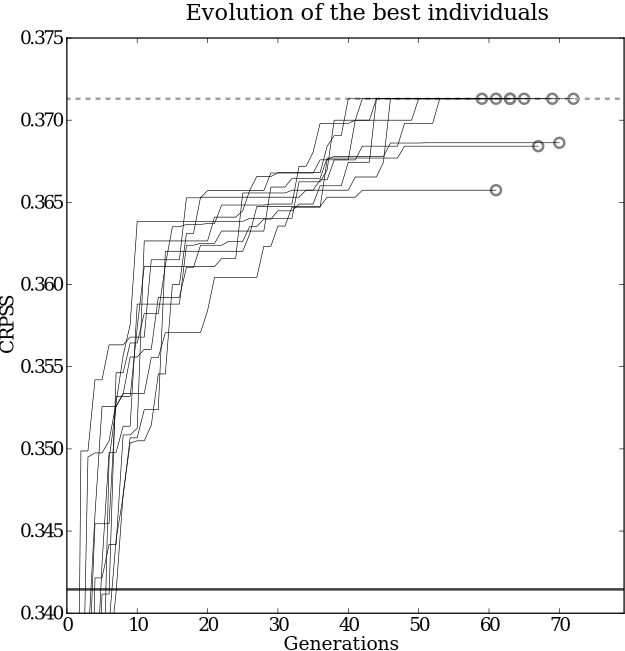
\includegraphics[width=19pc,angle=0]{figures/gas_evolution_good.pdf}\\
	\end{center}
	\caption{Evolution of the score of the best individuals over generations for the 10 optimizations processed for a given parametrization. The green line represents the score of the sequential approach and the blue one, the supposed global optimum.}
	\label{fig:gas_evolution_good}
\end{figure}


\begin{figure}[htb]
	\begin{center}
		\noindent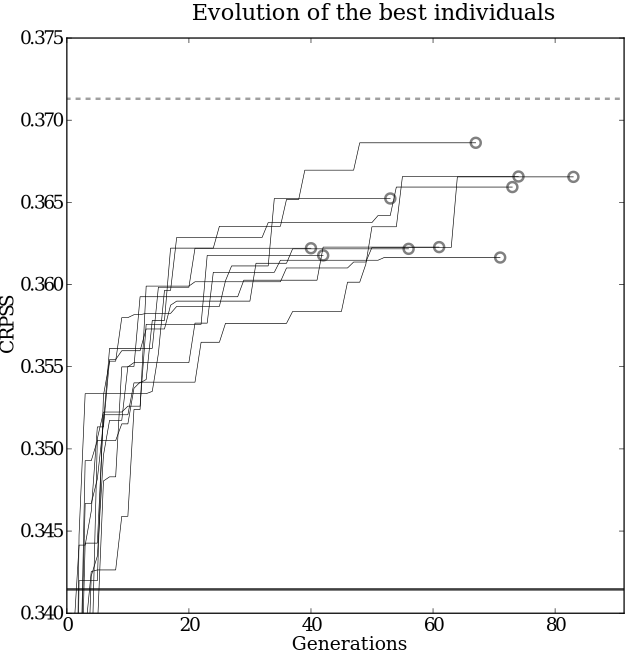
\includegraphics[width=19pc,angle=0]{figures/gas_evolution_bad.pdf}\\
	\end{center}
	\caption{Same as Figure \ref{fig:gas_evolution_good}, but for a GAs parametrization considered as less relevant.}
	\label{fig:gas_evolution_bad}
\end{figure}



\subsection{Results}

The results illustrate the effect of an operator when its contribution is isolated from the other operators. It means that we compare the effect of the studied operator when all the other operators are equivalent, while assessing multiple combinations. We then summarizes this contribution relatively to the other options, as a percentage of gain/loss regarding the mean of all variants. For example, to evaluate the performance of the uniform crossover operator, we compare some indicators between its performance and the average of performance of all crossover operators while retaining the same population size, the same mutation operators, natural selection, and selection of couples.

\subsubsection{Breeding operators}

We evaluated every combination of 6 options for the couples selection (Table \ref{tab:assessed_couples_selection_operators}) and 21 for the chromosome crossover operators (Table \ref{tab:assessed_crossover_operators}), along with variants of the other operators. This results in 1,008 combinations, requiring 10,080 optimizations.

\begin{table}[htbp]
	\caption{Assessed operator for couples selection.}
	\begin{center}
		\begin{tabular}{ll}
			\hline\hline  & \textbf{Couples selection operators} \\ 
			\hline 
			A & Rank pairing \\ 
			B & Random pairing \\ 
			C & Roulette wheel weighting on rank \\ 
			D & Roulette wheel weighting on fitness \\ 
			E & Tournament selection (3 candidates) \\ 
			F & Tournament selection (4 candidates) \\ 
			\hline 
		\end{tabular}
	\end{center}
	\label{tab:assessed_couples_selection_operators}
\end{table}

\begin{table}[htbp]
	\caption{Assessed operators for chromosome crossover.}
	\begin{center}
		\begin{tabular}{ll}
			\hline\hline  & \textbf{Chromosome crossover operators} \\ 
			\hline 
			1 & Single-point crossover \\
			2 & Two-point crossover \\
			3 & Multiple-point crossover (3 points) \\
			4 & Multiple-point crossover (5 points) \\
			5 & Uniform crossover \\
			6 & Blending method (2 points, unshared $\beta$) \\
			7 & Blending method (4 points, unshared $\beta$) \\
			8 & Blending method (2 points, shared $\beta$) \\
			9 & Blending method (4 points, shared $\beta$) \\
			10 & Linear crossover (2 points) \\
			11 & Linear crossover (4 points) \\
			12 & Heuristic crossover (2 points, unshared $\beta$) \\
			13 & Heuristic crossover (4 points, unshared $\beta$) \\
			14 & Heuristic crossover (2 points, shared $\beta$) \\
			15 & Heuristic crossover (4 points, shared $\beta$) \\
			16 & Binary-like crossover (2 points, unshared $\beta$) \\
			17 & Binary-like crossover (4 points, unshared $\beta$) \\
			18 & Binary-like crossover (2 points, shared $\beta$) \\
			19 & Binary-like crossover (4 points, shared $\beta$) \\
			20 & Linear interpolation \\
			21 & Free interpolation \\
			\hline
		\end{tabular}
	\end{center}
	\label{tab:assessed_crossover_operators}
\end{table}

After this first assessment, the importance of the mutation operator was obvious \cite[see][for the details]{Horton2012a}, and its leading influence on the optimization performance was evident. However, the effect of the operators and options other than the ones related to breeding will be detailed later.

\begin{figure}[htb]
	\begin{center}
		\noindent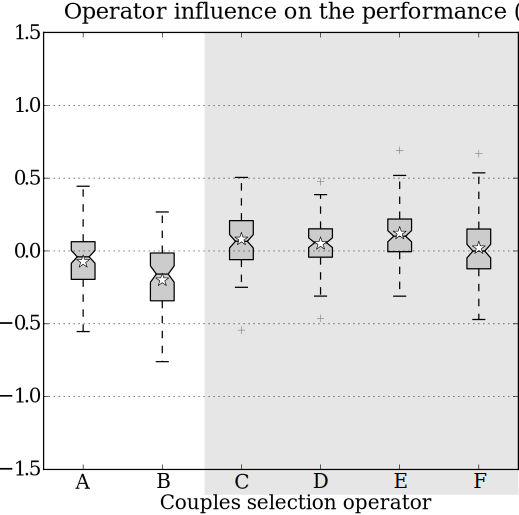
\includegraphics[width=7cm,angle=0]{figures/operator_selectcoupl_score.pdf}\\
	\end{center}
	\caption{Influence of the couples selection operators (Table \ref{tab:assessed_couples_selection_operators}) on the optimization performance. The box extends from the lower to upper quartile values of the data, with a line at the median. The whiskers extend from the box to 1.5 times the interquartile range. Flier points are those past the end of the whiskers. The star represents the median. The gray box highlights the best options.}
	\label{fig:operator_selectcoupl_score}
\end{figure}


\begin{figure*}[htb]
	\begin{center}
		\noindent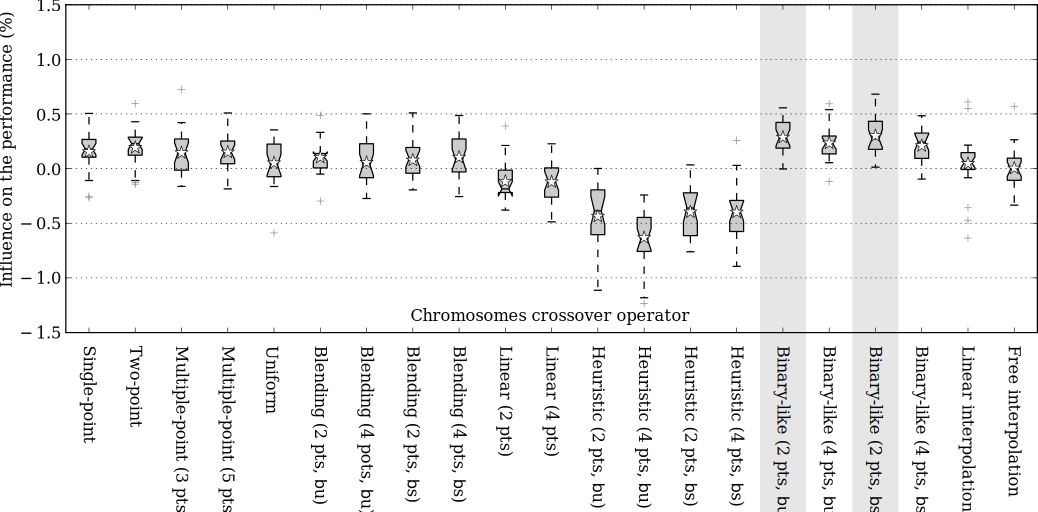
\includegraphics[width=16cm,angle=0]{figures/operator_crossover_score.pdf}\\
	\end{center}
	\caption{Influence of the chromosome crossover operators (Table \ref{tab:assessed_crossover_operators}) on the optimization performance. Same conventions as Figure \ref{fig:operator_selectcoupl_score}.}
	\label{fig:operator_crossover_score}
\end{figure*}

The performance of the couples selection operator are relatively close (Figure \ref{fig:operator_selectcoupl_score}). Overall, we observe that the random pairing performed the most poorly, whereas the tournament selection with 3~candidates is slightly superior to others. The roulette wheel weighting is almost equivalent, but is a bit less effective in terms of convergence and number of evaluations (not shown). This operator has not a significant role in our application. 

Analysis of crossover operators (Figure \ref{fig:operator_crossover_score}) reveal some slightly superior options, some inappropriate, and many averages. Among the inappropriate operators, we find first the heuristic crossover, which is also more demanding in terms of evaluation number, as well as the linear crossover. Binary-like crossover (especially with 2 points of intersection, whether $\beta$ is shared or not) are significantly better than the others, especially in terms of convergence (not shown). The two-point crossover is also relatively close. Other operators can also be considered usable.
	

\subsubsection{Mutation operator}

Having identified the leading role of the mutation operator, we strongly focused the sensitivity analysis on this operator. Each of the 10 different implementations (see section \ref{sec:gas:mutation}) was tested, with different parameters for those who require some (Table \ref{tab:assessed_mutation_operators}), bringing the number of variations of this operator up to 109. We also did some optimizations without any mutation as a reference. Along with variants of the other operators \citep[see][for the details]{Horton2012a}, it resulted in 660 combinations (so 6,600 optimizations).

\begin{table}[htbp]
	\caption{Assessed mutation operators with the number of variants considered (combination of parameters).}
	\begin{center}
		\begin{tabular}{llc}
			\hline\hline  & \textbf{Mutation operator} & \textbf{Variants}\\ 
			\hline 
			1 & Uniform mutation & 3 \\
			2 & Variable uniform mutation & 27 \\
			3 & Constant normal mutation & 9 \\
			4 & Variable normal mutation & 36 \\
			5 & Non-uniform mutation & 27 \\
			6 & Individual adaptive mutation rate & 1 \\
			7 & Individual adaptive search radius & 1 \\
			8 & Chromosome of adaptive mutation rate & 1 \\
			9 & Chromosome of adaptive search radius & 1 \\
			10 & Mutli-scale mutation & 3 \\
			11 & No mutation & 1 \\
			\hline
		\end{tabular}
	\end{center}
	\label{tab:assessed_mutation_operators}
\end{table}


\begin{figure}[htb]
	\begin{center}
		\noindent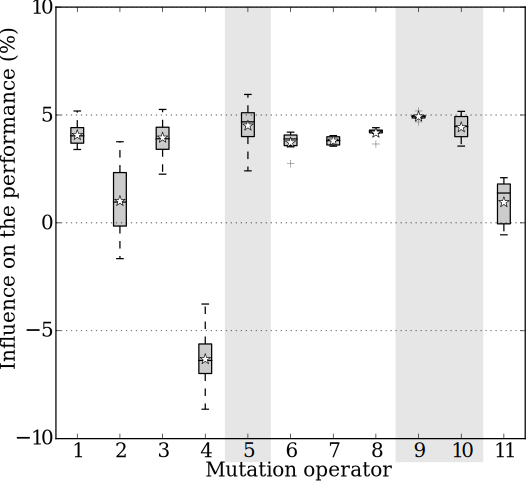
\includegraphics[width=7cm,angle=0]{figures/operator_mutation_score.pdf}\\
	\end{center}
	\caption{Influence of the mutation operators (Table \ref{tab:assessed_mutation_operators}) on the optimization performance. Same conventions as Figure \ref{fig:operator_selectcoupl_score}.}
	\label{fig:operator_mutation_score}
\end{figure}


Figure \ref{fig:operator_mutation_score} show the results of this analysis and illustrates the important role of the mutation on the performance of the optimizations. Optimizations without mutation (last box on the Figure) are inferior to most mutation operators, and the scale of the influence of the mutation operators is significantly more important than those for the other options. The details of the analysis \citep[see][]{Horton2012a} show that the other reproduction operators seem of secondary importance. This observation is in line with the work of \citet{Back1996a}, who argues for the importance of mutation over reproduction. He even suggests, in opposition with the theory of \citet{Holland1992a}, that chromosomes crossovers have mostly a corrective role of mutation operations. Various studies have also identified the importance of the mutation operator relatively to reproduction \citep[see eg.][]{Back1992a, Back1996b, Smith1997a, Deb1999, Haupt2004, Costa2005a, Costa2007a}.

The mutation operators based on a variable normal or uniform law work very poorly and are difficult to configure. We then observe many operators more or less with the same performance scores and requiring a variable amount of assessments. The convergence analysis \citep[see][]{Horton2012a} allows us to highlight three best operators: non-uniform mutation, chromosome of adaptive search radius, and multi-scale mutation. Because of the importance of the mutation operator on the resulting performance, we studied its role and parametrization in more detail. Thus, we performed different optimizations using variants of these 3 operators (Table \ref{tab:assessed_mutation_operators_bis}).

\begin{table}[htbp]
	\caption{Further assessments of mutation operators.}
	\begin{center}
		\begin{tabular}{llrrr}
			\hline\hline  & \textbf{Mutation operator} & \textbf{$p_{mut}$} & \textbf{$G_{max}$} & \textbf{$\omega$}\\ 
			\hline 1 & Non-uniform mutation & 0.01 & 50 & 0.1 \\
			2 & Non-uniform mutation & 0.05 & 50 & 0.1 \\
			3 & Non-uniform mutation & 0.1 & 50 & 0.1 \\
			4 & Non-uniform mutation & 0.2 & 50 & 0.1 \\
			5 & Non-uniform mutation & 0.4 & 50 & 0.1 \\
			6 & Non-uniform mutation & 0.01 & 100 & 0.1 \\
			7 & Non-uniform mutation & 0.05 & 100 & 0.1 \\
			8 & Non-uniform mutation & 0.1 & 100 & 0.1 \\
			9 & Non-uniform mutation & 0.2 & 100 & 0.1 \\
			10 & Non-uniform mutation & 0.4 & 100 & 0.1 \\
			11 & Mutli-scale mutation &  0.01 &&\\
			12 & Mutli-scale mutation &  0.05 && \\
			13 & Mutli-scale mutation &  0.1 && \\
			14 & Mutli-scale mutation &  0.2 && \\
			15 & Mutli-scale mutation &  0.4 && \\
			16 & \multicolumn{4}{l}{Chromosome of adaptive search radius} \\
			\hline
		\end{tabular}
	\end{center}
	\label{tab:assessed_mutation_operators_bis}
\end{table}

\begin{figure*}[htb]
	\begin{center}
		\noindent\includegraphics[width=14cm,angle=0]{figures/operator_mutation_score_atmlevel.pdf}\\
	\end{center}
	\caption{Influence of the mutation operators (Table \ref{tab:assessed_mutation_operators_bis}) on the optimization performance, leaving the optimizer choose the pressure level of the atmospheric circulation analogy (single level of analogy). The predictand is precipitation over a subcatchment in the Swiss Alps (Binn-Simplon region). The red line represents the score of the sequential calibration and the blue line, the score of the optimization without automatic selection of the pressure levels. Same conventions as Figure \ref{fig:operator_selectcoupl_score}.}
	\label{fig:operator_mutation_score_atmlevel}
\end{figure*}

\begin{figure*}[htb]
	\begin{center}
		\noindent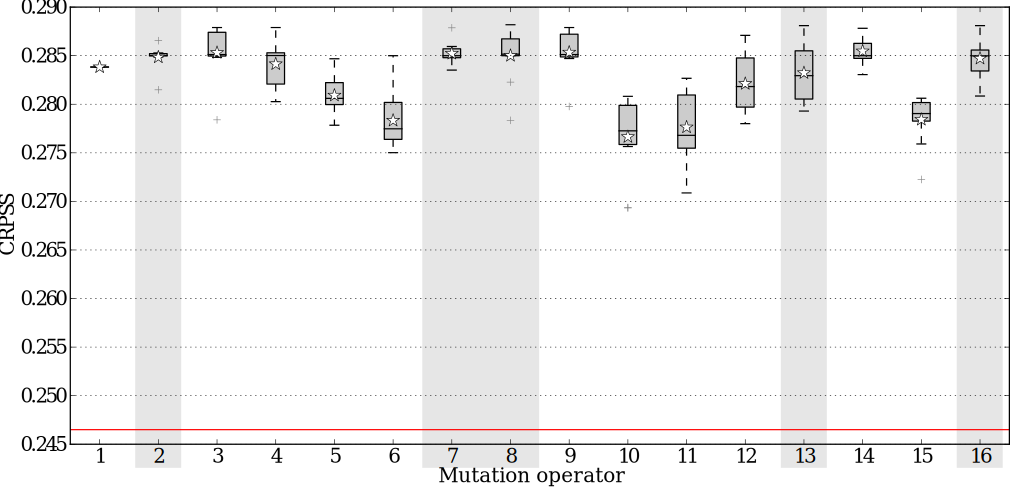
\includegraphics[width=14cm,angle=0]{figures/operator_mutation_score_rhoneamont.pdf}\\
	\end{center}
	\caption{Same as Figure \ref{fig:operator_mutation_score_atmlevel}, but for another region in the Swiss Alps (Bottom Rhone valley), with different atmospheric influences.}
	\label{fig:operator_mutation_score_rhoneamont}
\end{figure*}

\begin{figure*}[htb]
	\begin{center}
		\noindent\includegraphics[width=14cm,angle=0]{figures/operator_mutation_score_r2.pdf}\\
	\end{center}
	\caption{Same as Figure \ref{fig:operator_mutation_score_atmlevel}, but with a second level of analogy on moisture variables.}
	\label{fig:operator_mutation_score_r2}
\end{figure*}

\begin{figure*}[htb]
	\begin{center}
		\noindent\includegraphics[width=14cm,angle=0]{figures/operator_mutation_score_r4.pdf}\\
	\end{center}
	\caption{Same as Figure \ref{fig:operator_mutation_score_r2}, but with a preselection on air temperature rather than a fixed calendar window.}
	\label{fig:operator_mutation_score_r4}
\end{figure*}

The first analysis was the optimization of the precipitation forecasting over a subcatchment (Binn-Simplon region) in the Swiss Alps (Figure \ref{fig:operator_mutation_score_atmlevel}). The optimizer could choose the 2 pressure levels of the atmospheric circulation analogy (method with a single level of analogy). The resulting performance score is obviously superior to the one from the sequential calibration (red line on Figure \ref{fig:operator_mutation_score_atmlevel}). For most options, it is also slightly better than the results from the optimization without selection of the pressure levels (blue line). A clear breakthrough of the performances was not expected, as the former selection of pressure levels results from intensive work \citep{Bontron2004}. This application however demonstrates that, when correctly parametrized, GAs can automatically and successfully choose the pressure levels. However, some less relevant optimizations do not match the previous results. We could clearly observe, through different applications, that the automatic selection of the pressure level significantly increases the difficulty for GAs to converge to a unique solution, ideally the global optimum. A difficulty is that the pressure levels are considered within the optimization without continuity between values, and thus the approaches relying on distance in the parameters space, such as the search radius, cannot fully exploit the properties that make them efficient. However, even though the results show a certain variability, most of them present very good performance scores, despite different parameters of the AM. As illustrated in \cite{Horton2016}, the surface response of the parameters space of the AM is rather gentle in certain regions, meaning it allows for different values of some parameters without significantly impacting the performance score.

Then, we performed the same optimization, but for another region, sensitive to other meteorological influences (Figure \ref{fig:operator_mutation_score_rhoneamont}), in order to assess eventual dependencies of the operator with the predictand. Even though we can observe differences with Figure \ref{fig:operator_mutation_score_atmlevel}, it is globally the same options that perform better.

Next, we added a second level of analogy on moisture variables (Figure \ref{fig:operator_mutation_score_r2}). The optimizer had to optimize both levels of analogy simultaneously. Once again, despite the difficulty to optimize simultaneously both levels of analogy, the results were better than the sequential calibration (red line on Figure \ref{fig:operator_mutation_score_r2}). And finally, we added a preselection on air temperature instead of the fixed calendar window, as proposed by \cite{BenDaoud2010}. The results show generally higher scores (Figure \ref{fig:operator_mutation_score_r4}), demonstrating the success of the optimizer to take advantage of this new degree of liberty, and its capacity to handle optimization of 3 analogy levels jointly. Again, the most relevant options are generally the same.

After analysis of the most relevant mutation operators, we can raise the following advice (detailed parametrization are provided in section \ref{sec:recommendations}):

\begin{itemize}
	
	\item \textit{Non-uniform mutation} \citep{Michalewicz1996}: this operator is good in terms of convergence, mainly when the number of parameters to optimize is rather low. The number of required evaluations, however, can be quite substantial. The main disadvantage of the non-uniform mutation is the complexity of its parametrization, which is difficult to estimate a priori. These parameters must be carefully chosen to be in line with the evolution rate of the population, and are therefore dependent on the problem being treated. We could observe that the $\omega$ coefficient does not influence performance. The role of $G_{m}$ is rather difficult to judge, but does not seem essential. The mutation rate was found to be important. The difficulty is that the optimal value seems to be very case-related. Indeed, by even changing the precipitation time series (ie optimizing for another subregion), but not the complexity of the AM, the optimal mutation rate changes, making it impossible to estimate in advance.
	
	\item \textit{Chromosome of adaptive search radius} (new): unlike the previous one, our new operator is very robust, as it requires no option and is auto-adapting. It may be sometimes a little bit slower for simple problems, but does not require parametrization, which is an important advantage. It is interesting to notice that our insertion of an extra chromosome representing the search radius gives better performance than other self-adaptive operators (such as, for example, the chromosome of adaptive mutation rate). If one had to choose a single option for the mutation operator, we would recommend the chromosome of adaptive search radius, as it was proven effective and needs no parameter.
	
	\item \textit{Multi-scale mutation} (new): finally, our multi-scale mutation, which also performs pretty well, requires one parameter, the mutation rate. However, it can also be difficult to estimate a correct value a priori.
	
\end{itemize}

In our application, the mutation operator has a leading effect and should be chosen with care. It may be wise to perform multiple optimizations and to consider these three operators in parallel in order to obtain results from algorithms that are either sometimes more efficient or more robust. It is interesting to note that the three best techniques incorporate a notion of search distance. It is likely that this notion is the key to these algorithms, for our application, and allows them to initially explore the parameter domain, and then to converge. The search radius in fact directly represents the notion of transition between exploration and exploitation, in our opinion more than a possible evolution of mutation rates.


\subsubsection{Other options}

The analysis of the natural selection operator (Figure \ref{fig:operator_selectnat_score}) reveals a slight preference for the ratio-elitism compared to the tournament selection, but not so significant. Furthermore, the number of evaluations is similar. This operator, or at least the two assessed versions, do not appear to significantly influence the optimization performances.

\begin{figure}[htb]
	\begin{center}
		\noindent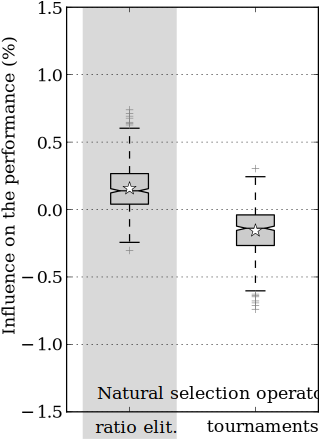
\includegraphics[width=4cm,angle=0]{figures/operator_selectnat_score.pdf}\\
	\end{center}
	\caption{Influence of the natural selection operators on the optimization performance. Same conventions as Figure \ref{fig:operator_selectcoupl_score}.}
	\label{fig:operator_selectnat_score}
\end{figure}

The size of the population ($N$) has an effect on the performance of the optimization (Figure \ref{fig:option_taillepop_score}). A bigger population leads to better results, but also to significantly longer optimizations. Indeed, the required number of evaluation, and thus the required time, is approximately proportional to the population size. The optimal size seems to depend on the complexity of the AM to optimize: a more complex AM (ie. with more degrees of freedom) requires a bigger population size. A rule of thumb based on different experiences (not shown here) is provided hereafter:

\begin{itemize}
	\item $50<N\leqslant100$ for a very simple implementation of the AM (1 level of analogy with 2 pressure levels),
	\item $N\approx200$ for a bit more complex AM (1 level of analogy with 4 pressure levels, or 2 level of analogy with less pressure levels),
	\item $N\approx500$ for significantly more complex AMs (2-3 levels of analogy with 4 pressure levels for the atmospheric circulation, and 2 to 4 levels for the moisture analogy).
\end{itemize}

We didn't find any improvement with $N>500$, the results were even surprisingly of a lower quality. However, this relies on a limited number of case studies and cannot be generalized. It depends on the AM to optimize, and supposedly on the characteristics of the processes generating the precipitations in a given region. 

\begin{figure}[htb]
	\begin{center}
		\noindent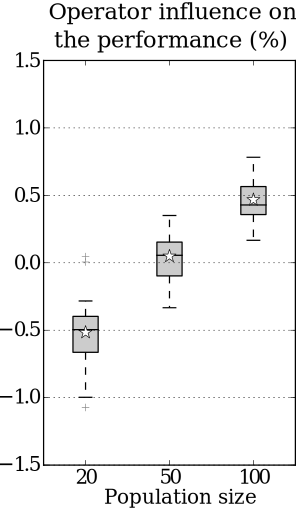
\includegraphics[width=4cm,angle=0]{figures/option_taillepop_score.pdf}\\
	\end{center}
	\caption{Influence of the population size on the optimization performance. Same conventions as Figure \ref{fig:operator_selectcoupl_score}.}
	\label{fig:option_taillepop_score}
\end{figure}

We also assessed the influence of the size of the intermediate population (ratio of the total population) selected for mating (Figure \ref{fig:option_popratio_score}). It appears that a big ratio is not optimal. However, it does not appear that this parameter is critical to the quality of the optimizations, provided it is not too big. A value of 50~\% seems a wise choice.

\begin{figure}[htb]
	\begin{center}
		\noindent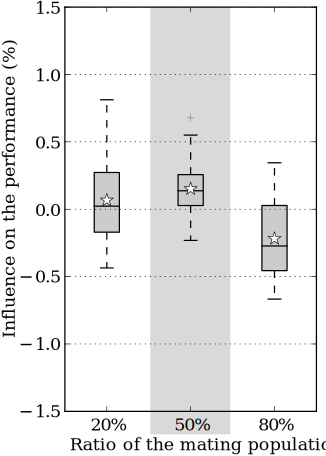
\includegraphics[width=4cm,angle=0]{figures/option_popratio_score.pdf}\\
	\end{center}
	\caption{Influence of the intermediate population ratio on the optimization performance. Same conventions as Figure \ref{fig:operator_selectcoupl_score}.}
	\label{fig:option_popratio_score}
\end{figure}


\section{Recommended parametrization of GAs}
\label{sec:recommendations}

We evaluated the optimization by genetic algorithms on AMs of varying complexity, with a large number of combinations of operators to be able to make recommendations for optimizing the AM. Our conclusions are:

\begin{itemize}
	\item The optimization does not systematically converge to the global optimum  (but still often nearby), which is why we recommend doing several optimizations in parallel in order to compare the results, analyse the convergence, and keep the best.
	
	\item The population size should be in accordance with the complexity of the AM to optimize: from 50 for the simple ones, up to 500 for the most complex AMs.
	
	\item The value of the ratio for the intermediate population is not so important, and value of 50\% seems quite appropriate.
	
	\item Ratio-elitism is slightly better than tournaments for the natural selection operator, but it is not decisive.
	
	\item The performance of the operators for the couples selection perform relatively similarly. The roulette wheel weighting and the tournament selection are more efficient in terms of convergence and required number of evaluations.
	
	\item Most crossover operators have relatively similar performance. Binary-like crossover with two points of intersection are better than others, especially for convergence.
	
	\item Mutation has a clearly dominant influence. Three mutation operators stand out, two of which we have developed: the non-uniform mutation, the multi-scale mutation, and the chromosome of adaptive search radius. The latter is the most robust as it has no controlling parameter.
	
\end{itemize}

In order to make an optimization of the AM with genetic algorithms, it may be wise to consider these three mutation operators in parallel. We would then combine algorithms that are sometimes faster to other that are more robust. In order to be confident in the optimized AMs, we propose using a set of the following mutation operators:

\begin{itemize}
	\setlength\itemsep{-4px}
	\item 1x non-uniform, $p_{mut}=0.05$, $G_{m}=50$, $\omega=0.1$
	\item 1x non-uniform, $p_{mut}=0.05$, $G_{m}=100$, $\omega=0.1$
	\item 1x non-uniform, $p_{mut}=0.1$, $G_{m}=100$, $\omega=0.1$
	\item 1x multi-scale,  $p_{mut}=0.1$
	\item 2x chromosome of adaptive search radius
\end{itemize}


\section{Conclusions}


In order to automatically optimize the analogue method, we evaluated genetic algorithms, a global optimization technique, that is able to solve complex problems. Given the large number of existing operators and options, we had to evaluate systematically multiple variants to identify which operators are important, and which variant works best for the analogue method. We could thus identify that the mutation operator is a key element for our application, and provided new variants that were found to be efficient, such as the Chromosome of adaptive search radius that seems to be very reliable (no control parameter) and efficient . Recommendations were established for a relevant use of GAs for the optimization of the analogue method. However, there may still be possible improvements, through new operators, in order to improve the optimization performance and speed. Usage of this global optimization greatly eases the adaptation of the AM to new regions (with different leading meteorological processes) or to new predictands, as the optimization is performed automatically and globally.





The global optimization tools allow easily adapting the AM to new regions by taking into account local meteorological influences, and has thus a great potential of use. Moreover, it allows exploring automatically datasets in order to extract the most relevant variables. It is thus possible to try assessing other predictands, such as the temperature, the limit of snowfall, the occurrence of hail, or wind, while leaving the algorithms select the best variables and the associated parameters.


%%%%%%%%%%%%%%%%%%%%%%%%%%%%%%%%%%%%%%%%%%%%%%%%%%%%%%%%%%%%%%%%%%%%%
% ACKNOWLEDGMENTS
%%%%%%%%%%%%%%%%%%%%%%%%%%%%%%%%%%%%%%%%%%%%%%%%%%%%%%%%%%%%%%%%%%%%%
%
\acknowledgments
Thanks to Hamid Hussain-Khan of the University of Lausanne for his help and availability, and for the intensive use of the cluster he is in charge of. Thanks to Renaud Marty for his fruitful collaboration over the years.

Thanks to the Swiss Federal Office for Environment (FOEV), the Roads and Water courses Service, Energy and Water Power Service of the Wallis Canton and the Water, Land and Sanitation Service of the Vaud Canton who financed the MINERVE (Mod\'{e}lisation des Intemp\'{e}ries de Nature Extr\^{e}me des Rivi\`{e}res Valaisannes et de leurs Effets) project which started this research. NCEP reanalysis data provided by the NOAA/OAR/ESRL PSD, Boulder, Colorado, USA, from their Web site at http://www.esrl.noaa.gov/psd/. Precipitation time series provided by MeteoSwiss. 


%%%%%%%%%%%%%%%%%%%%%%%%%%%%%%%%%%%%%%%%%%%%%%%%%%%%%%%%%%%%%%%%%%%%%
% APPENDIXES
%%%%%%%%%%%%%%%%%%%%%%%%%%%%%%%%%%%%%%%%%%%%%%%%%%%%%%%%%%%%%%%%%%%%%
%
% Use \appendix if there is only one appendix.
%\appendix

% Use \appendix[A], \appendix}[B], if you have multiple appendixes.
%\appendix[A]

%% Appendix title is necessary! For appendix title:
%\appendixtitle{}

%%% Appendix section numbering (note, skip \section and begin with \subsection)
% \subsection{First primary heading}

% \subsubsection{First secondary heading}

% \paragraph{First tertiary heading}

%% Important!
%\appendcaption{<appendix letter and number>}{<caption>} 
%must be used for figures and tables in appendixes, e.g.,
%
%\begin{figure}
%\noindent\includegraphics[width=19pc,angle=0]{figure01.pdf}\\
%\appendcaption{A1}{Caption here.}
%\end{figure}
%
% All appendix figures/tables should be placed in order AFTER the main figures/tables, i.e., tables, appendix tables, figures, appendix figures.
%
%%%%%%%%%%%%%%%%%%%%%%%%%%%%%%%%%%%%%%%%%%%%%%%%%%%%%%%%%%%%%%%%%%%%%
% REFERENCES
%%%%%%%%%%%%%%%%%%%%%%%%%%%%%%%%%%%%%%%%%%%%%%%%%%%%%%%%%%%%%%%%%%%%%
% Make your BibTeX bibliography by using these commands:
\bibliographystyle{ametsoc2014}
% \bibliography{references}
\bibliography{../_refs/_articles-gas}

%%%%%%%%%%%%%%%%%%%%%%%%%%%%%%%%%%%%%%%%%%%%%%%%%%%%%%%%%%%%%%%%%%%%%
% TABLES
%%%%%%%%%%%%%%%%%%%%%%%%%%%%%%%%%%%%%%%%%%%%%%%%%%%%%%%%%%%%%%%%%%%%%
%% Enter tables at the end of the document, before figures.
%%
%
%\begin{table}[t]
%\caption{This is a sample table caption and table layout.  Enter as many tables as
%  necessary at the end of your manuscript. Table from Lorenz (1963).}\label{t1}
%\begin{center}
%\begin{tabular}{ccccrrcrc}
%\hline\hline
%$N$ & $X$ & $Y$ & $Z$\\
%\hline
% 0000 & 0000 & 0010 & 0000 \\
% 0005 & 0004 & 0012 & 0000 \\
% 0010 & 0009 & 0020 & 0000 \\
% 0015 & 0016 & 0036 & 0002 \\
% 0020 & 0030 & 0066 & 0007 \\
% 0025 & 0054 & 0115 & 0024 \\
%\hline
%\end{tabular}
%\end{center}
%\end{table}




%%%%%%%%%%%%%%%%%%%%%%%%%%%%%%%%%%%%%%%%%%%%%%%%%%%%%%%%%%%%%%%%%%%%%
% FIGURES
%%%%%%%%%%%%%%%%%%%%%%%%%%%%%%%%%%%%%%%%%%%%%%%%%%%%%%%%%%%%%%%%%%%%%
%% Enter figures at the end of the document, after tables.
%%
%
%\begin{figure}[t]
%  \noindent\includegraphics[width=19pc,angle=0]{figure01.pdf}\\
%  \caption{Enter the caption for your figure here.  Repeat as
%  necessary for each of your figures. Figure from \protect\cite{Knutti2008}.}\label{f1}
%\end{figure}





\end{document}